% Options for packages loaded elsewhere
\PassOptionsToPackage{unicode}{hyperref}
\PassOptionsToPackage{hyphens}{url}
%
\documentclass[
]{article}
\usepackage{amsmath,amssymb}
\usepackage{iftex}
\ifPDFTeX
  \usepackage[T1]{fontenc}
  \usepackage[utf8]{inputenc}
  \usepackage{textcomp} % provide euro and other symbols
\else % if luatex or xetex
  \usepackage{unicode-math} % this also loads fontspec
  \defaultfontfeatures{Scale=MatchLowercase}
  \defaultfontfeatures[\rmfamily]{Ligatures=TeX,Scale=1}
\fi
\usepackage{lmodern}
\ifPDFTeX\else
  % xetex/luatex font selection
\fi
% Use upquote if available, for straight quotes in verbatim environments
\IfFileExists{upquote.sty}{\usepackage{upquote}}{}
\IfFileExists{microtype.sty}{% use microtype if available
  \usepackage[]{microtype}
  \UseMicrotypeSet[protrusion]{basicmath} % disable protrusion for tt fonts
}{}
\makeatletter
\@ifundefined{KOMAClassName}{% if non-KOMA class
  \IfFileExists{parskip.sty}{%
    \usepackage{parskip}
  }{% else
    \setlength{\parindent}{0pt}
    \setlength{\parskip}{6pt plus 2pt minus 1pt}}
}{% if KOMA class
  \KOMAoptions{parskip=half}}
\makeatother
\usepackage{xcolor}
\usepackage{graphicx}
\makeatletter
\def\maxwidth{\ifdim\Gin@nat@width>\linewidth\linewidth\else\Gin@nat@width\fi}
\def\maxheight{\ifdim\Gin@nat@height>\textheight\textheight\else\Gin@nat@height\fi}
\makeatother
% Scale images if necessary, so that they will not overflow the page
% margins by default, and it is still possible to overwrite the defaults
% using explicit options in \includegraphics[width, height, ...]{}
\setkeys{Gin}{width=\maxwidth,height=\maxheight,keepaspectratio}
% Set default figure placement to htbp
\makeatletter
\def\fps@figure{htbp}
\makeatother
\setlength{\emergencystretch}{3em} % prevent overfull lines
\providecommand{\tightlist}{%
  \setlength{\itemsep}{0pt}\setlength{\parskip}{0pt}}
\setcounter{secnumdepth}{-\maxdimen} % remove section numbering
\ifLuaTeX
  \usepackage{selnolig}  % disable illegal ligatures
\fi
\usepackage{bookmark}
\IfFileExists{xurl.sty}{\usepackage{xurl}}{} % add URL line breaks if available
\urlstyle{same}
\hypersetup{
  hidelinks,
  pdfcreator={LaTeX via pandoc}}

\author{}
\date{}

\begin{document}

\section{Pipeline of analysis}\label{pipeline-of-analysis}

Note: some tasks are more computationally intense than others and more
complicated; their location is in the \emph{scripts} folder.
Tasks/scripts are lightweight; they will be in ``example code'' in this
document except were noted. Change the example code to fit your file's
location/directory/naming.

The figure below show the pipeline of analysis with the rectangle boxes
equivalent to the sections in this README.
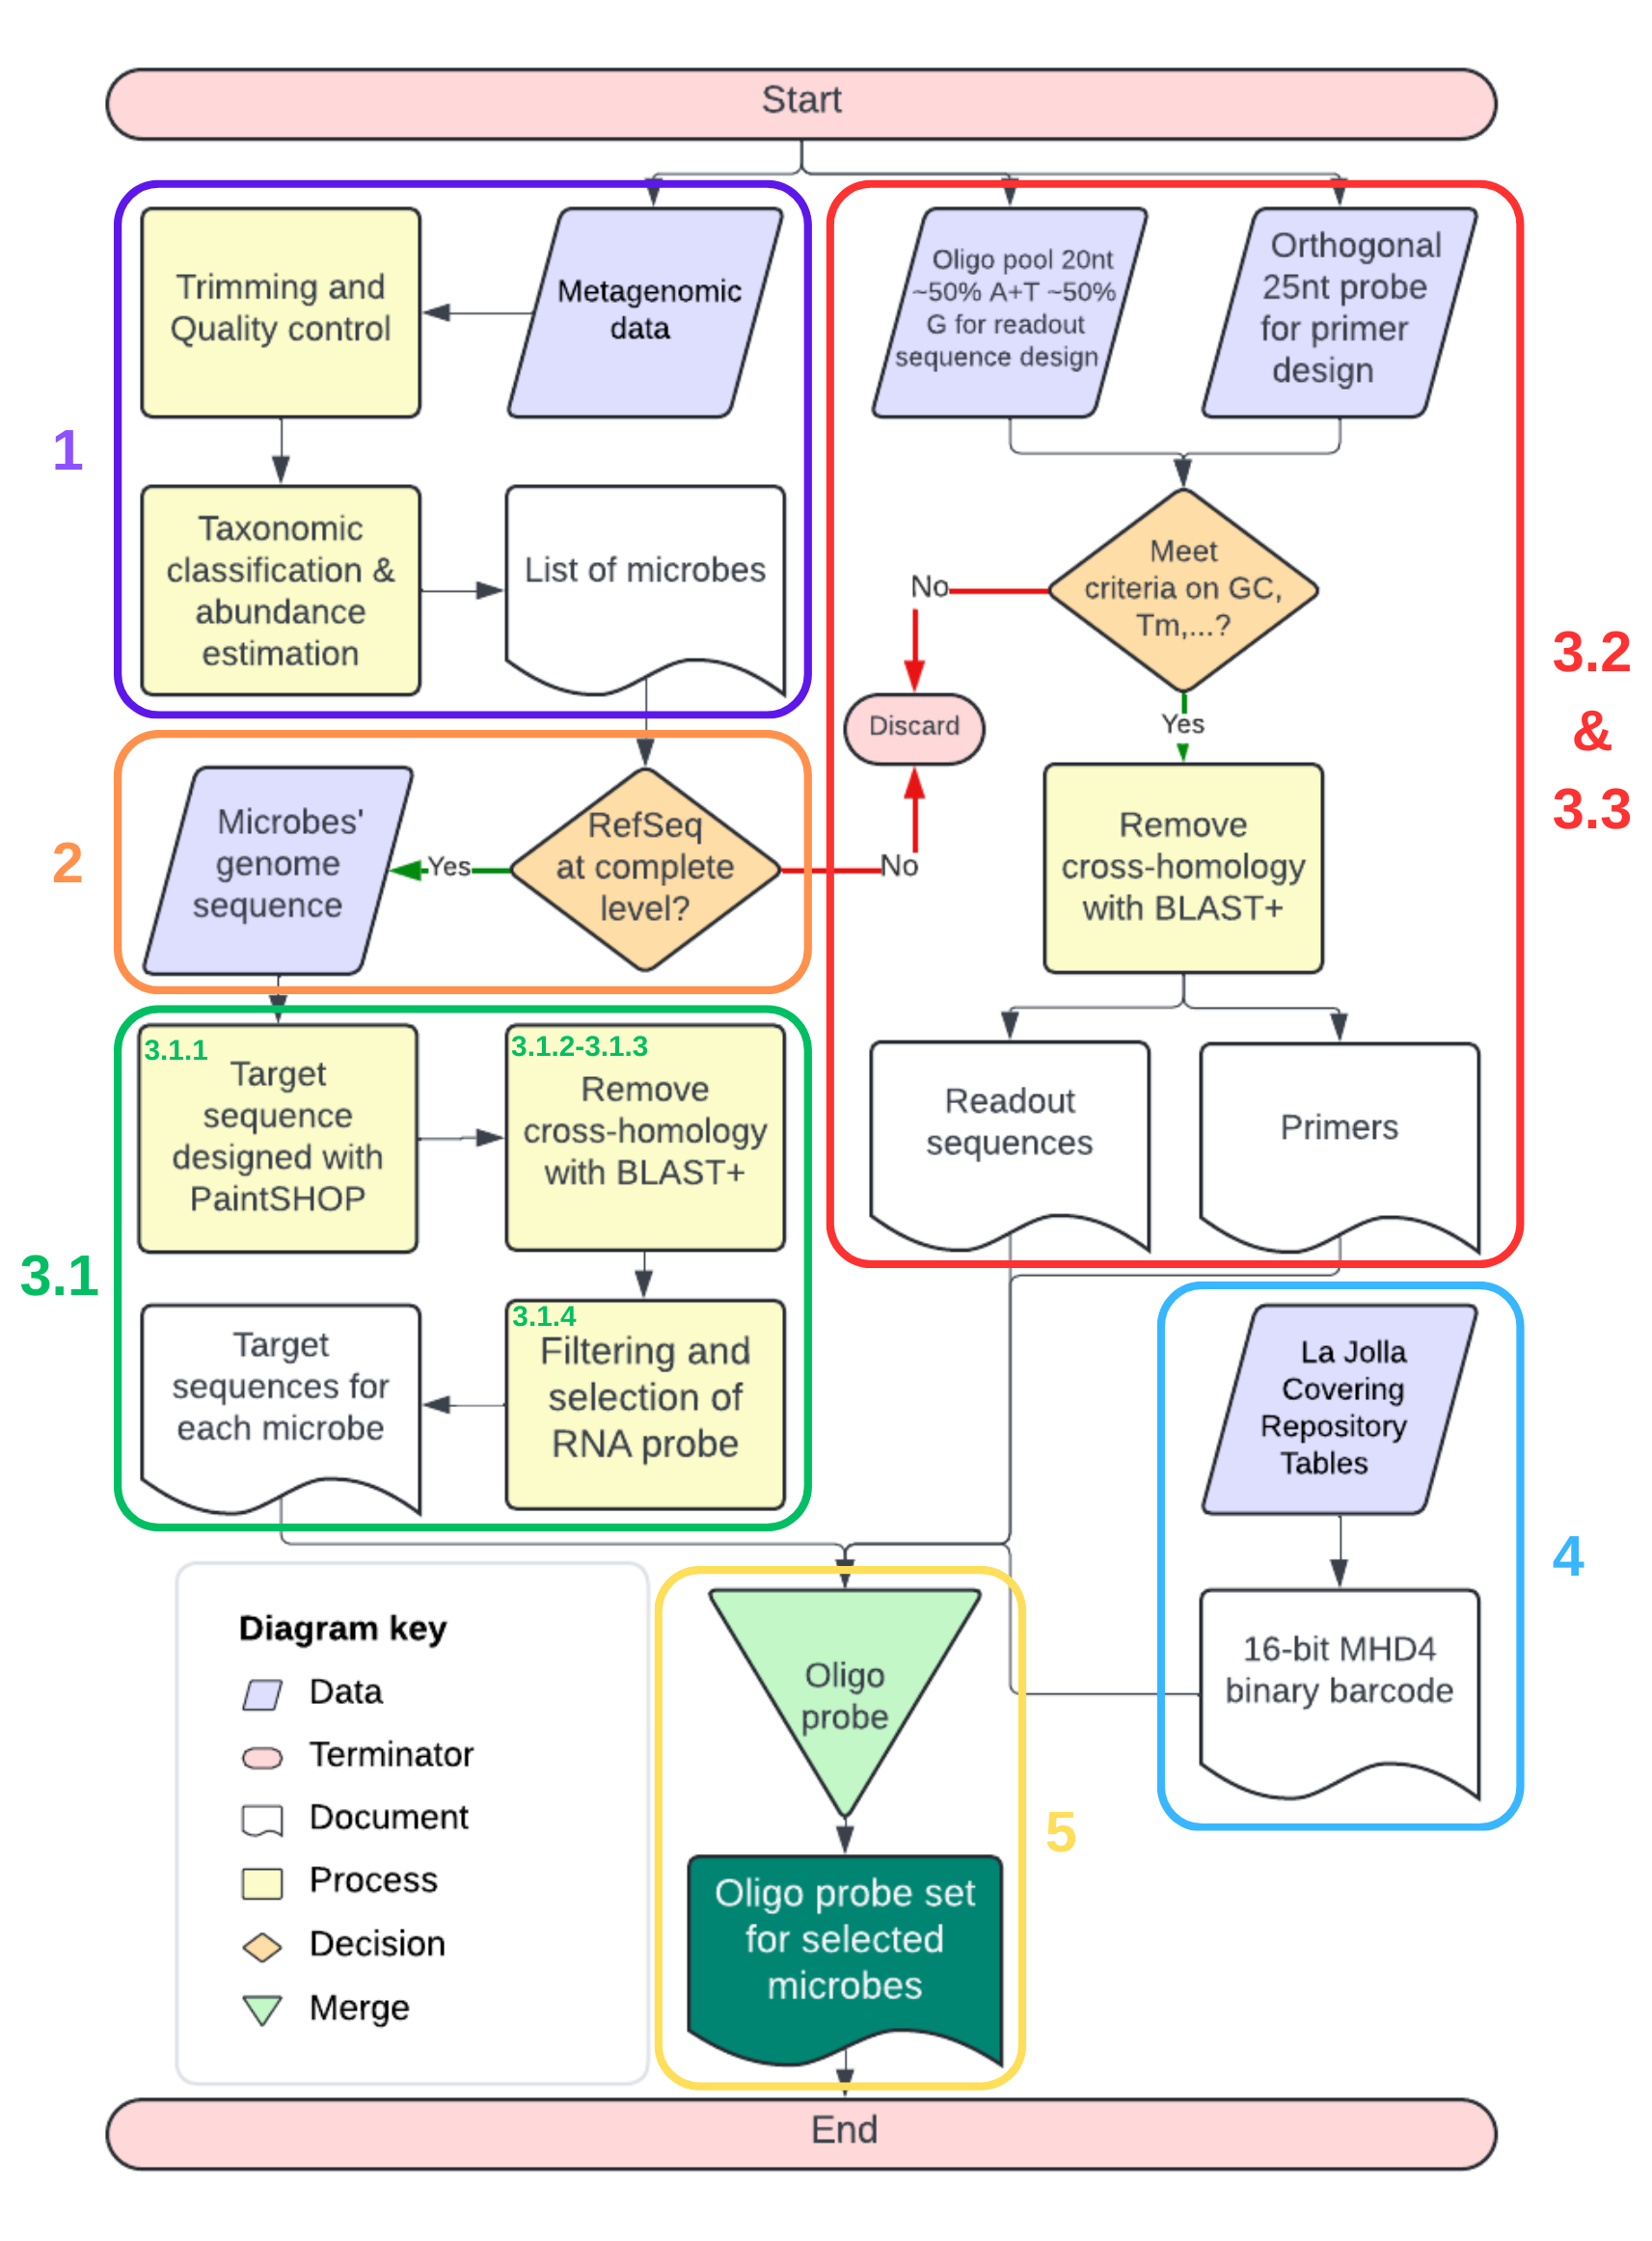
\includegraphics{https://github.com/npxhuy/MERFISH_probeDesign/blob/main/figure/flowchart_MD.png}

\subsection{1. Classification of Microbes and Abundance
estimation.}\label{classification-of-microbes-and-abundance-estimation.}

\href{https://biorg.cs.fiu.edu/Smoking/}{Metagenomics data}
(RawData-CamposEtAl.zip) was taken from
\href{https://www.microbiologyresearch.org/content/journal/acmi/10.1099/acmi.0.000497.v3\#R52}{this
paper}. The classification of microbes is done using the same pipeline
from \href{https://github.com/npxhuy/microbiome}{my previous project}.
Please refer to that GitHub link to do this step.

For short 1. You must QC the metagenomic data with FastQC for
decision-making. You can skip the trimming step if the data gives good
results with FastQC.

\begin{enumerate}
\def\labelenumi{\arabic{enumi}.}
\setcounter{enumi}{1}
\item
  You will need to run Kraken2 on the trimmed data. You can always make
  your database if you do not want to use the PlusPF database. To build
  a database, please refer to Kraken2
  \href{https://github.com/DerrickWood/kraken2/blob/master/docs/MANUAL.markdown}{manual}.
\item
  You will need to run Bracken on the Kraken2 results. If you make your
  database for Bracken, you need to build the Bracken k-mer database
  within your database. Please refer to Bracken
  \href{https://github.com/jenniferlu717/Bracken}{manual}\\
  Having the classification of microbes, the first column of every
  bracken report is the name of species, cut them out and put them in a
  file, which will be used later on.
\end{enumerate}

\subsection{2. Raw data processing}\label{raw-data-processing}

Now that you have the list of microbes, you can download their genome
from NCBI, for example. If you can find an alternative way to download
microbe data, it's good for you; if you already have them, it's also
good for you. If not, use
\href{https://www.ncbi.nlm.nih.gov/datasets/docs/v2/download-and-install/}{datasets
command-line tools} to download the FASTA and GTF file of the microbes
from NCBI. For this research, we used PaintSHOP to design target probes
using FASTA and GTF files. Example code for this task is
\emph{download\_data.sh}. You will need the microbes list from
\textbf{1} for this task.

The genome files are in zip format; unzip them! GTF files have bunches
of lines starting with \#, which can prevent PaintSHOP from running;
remove it.

Example code:
\texttt{ls\ \textbar{}\ while\ read\ folder;\ cd\ \$folder/ncbi\_dataset/data/*/;\ do\ grep\ -v\ "\#"\ genomic.gtf\ \textgreater{}\ genomic.tmp\ \&\&\ mv\ genomic.tmp\ genomic.gtf;\ cd\ ../../../..;\ done}

The folder and naming are pretty tricky because of multiple folders and
using accession numbers instead of scientific names for the FASTA and
GTF files, which were all named genomic.gtf. To make it easier, you can
soft-link them to another folder.

Example code:
\texttt{ls\textbar{}\ while\ read\ microbes;\ do\ cd\ \$microbes;\ ln\ -s\ ../../01\_unzip\_data/\$microbes/ncbi\_dataset/data/*/*.fna\ \$microbes.fna;\ ln\ -s\ ../../01\_unzip\_data/\$microbes/ncbi\_dataset/data/*/*.gtf\ \$microbes.gtf;\ cd\ ..;\ done}

\subsection{3. Probe design}\label{probe-design}

\subsubsection{3.1 Target sequence}\label{target-sequence}

\paragraph{3.1.1 Probe design}\label{probe-design-1}

\href{https://github.com/beliveau-lab/PaintSHOP_pipeline}{PaintSHOP\_pipeline}
was used to perform probe design. Follow the instructions on their
GitHub to run the pipeline. The pipeline was run on a loop repeatedly on
all microbes' data.

The melting temperature, length of probes, and other settings need to be
stated in the config.yml file. See the script \emph{paintshop\_loop.sh}
for more info. This is a modified script base on their
\emph{run\_pipeline.sh} script, to make it into a loop and write
config.yml file for every species, that's the fundamental of the
scripts, in case it's not working with you device, I suffered it too.

The error may occur when you give a high Tm with a short probe length,
making the tool unable to produce any probes. With that Tm and length,
some probes can satisfy the input. You can consider separating the code
into two parts: generating a config.yml file for all the microbes and
running PaintSHOP on the data for a less complicated task.

Example of output: \textgreater{} NZ\_CP043953.1 174 203
ATTGGCTGAACAATTGTCAGAAGGGCGGGT 42.480 100.000 0.000 0 0.307 0 +\\
NZ\_CP043953.1 256 285 AGTGAACAGCCTGCAACAACTACAGCAGCT 42.260 96.458
0.000 0 0.285 0 +\\
NZ\_CP043953.1 417 446 TGAAGGCCGTTCTAACCAAATGGCAGCAGA 42.200 100.000
0.000 0 0.265 0 +

\paragraph{3.1.2 Make databases for
blastn}\label{make-databases-for-blastn}

The probe was screened against the human genome and with other microbes
with
\href{https://blast.ncbi.nlm.nih.gov/doc/blast-help/downloadblastdata.html}{Blast+}.
To run Blast+, we need a blast database of that genome.

Download a version that fits your current platform, and we can start
with the making of the database using makeblastdb tool. For this step,
two main db will be made: 1. human genome, 2. microbes genome.

\begin{enumerate}
\def\labelenumi{\arabic{enumi}.}
\item
  Human genome database\\
  Download the fasta file from
  \href{https://www.ncbi.nlm.nih.gov/genome/guide/human/}{here}. Extract
  the file if needed and run \emph{makeblastdb} on it.\\
  Example code:
  \texttt{makeblastdb\ -in\ \$human.fasta\ -dbtype\ nucl\ -out\ \$human\_db}
\item
  Microbe genome database\\
  To run screen one speice to all other species other than that species,
  we need to combine the data of other species and then
  \emph{makeblastdb}
\end{enumerate}

\begin{itemize}
\tightlist
\item
  Example code of combine fasta file: check
  \emph{combine\_fasta\_for\_makeblastdb.sh}
\item
  Example code of \emph{makeblastdb} on the combined fasta file: check
  \emph{makeblastdb\_microbe.sh}
\end{itemize}

\paragraph{3.1.3 Screening with blastn +
filtering}\label{screening-with-blastn-filtering}

This step will be repeated many times. When we have the database, we run
blastn to screen the probe on the database. Having the blastn result, we
parse it, extract the found sequences (which means those sequences are
not unique) and filter it back to the original file.

\begin{enumerate}
\def\labelenumi{\arabic{enumi}.}
\tightlist
\item
  Make the probes result in fasta format.\\
  Example code:
  \texttt{cat\ \$probe\_result.tsv\ \textbar{}\ cut\ -f4\ \textbar{}\ awk\ \textquotesingle{}\{print\ "\textgreater{}\textbackslash{}n"\$0\}\textquotesingle{}\ \textgreater{}\ \$probe\_result.fasta}\\
  Example output: \textgreater{} \textgreater{}\\
  ATTGGCTGAACAATTGTCAGAAGGGCGGGT\\
  \textgreater{}\\
  AGTGAACAGCCTGCAACAACTACAGCAGCT\\
  \textgreater{}\\
  TGAAGGCCGTTCTAACCAAATGGCAGCAGA
\item
  Run blastn. This could be heavy in term of computational resources,
  but not at this step yet.\\
  Example
  code:\texttt{blastn\ -db\ \$db\_name\ -query\ \$probe\_result.fasta\ -word\_size\ \$number\ -ungapped\ \textgreater{}\ \$blast\_result\_file}
\item
  Parse blast result.\\
  Example code:
  \texttt{grep\ "Sbjct"\ -B\ 2\ \$blast\_result\_file\ \textbar{}\ grep\ "Query"\ \textbar{}\ awk\ \textquotesingle{}\{print\ \$3\}\textquotesingle{}\ \textbar{}\ sort\ \textbar{}\ uniq\ \textbar{}\ grep\ -v\ -f\ -\ \$probe\_result.fasta\ \textbar{}\ grep\ -v\ "\textgreater{}"\ \textgreater{}\ \$unique\_probe}
\item
  (Optional if you want to repeat the process) Change the
  \$unique\_probe to fasta format.\\
  Example code:
  \texttt{awk\ \textquotesingle{}\{print\ "\textgreater{}\textbackslash{}n"\$0\}\textquotesingle{}\ \$unique\_probe\ \textgreater{}\ \$unique\_probe.fasta}
\end{enumerate}

Run these steps to screen the human genome, obtaining the probes that
are unique to the human genome. Screen the unique probes on the human
genome on microbes genome, obtaining the unique probes on human +
microbes.

In step 2, technically, it can run normally with a single thread, taking
around 5-10 mins without using any additional core power. However, you
can utilise multiprocessing for faster time processing, which will be
helpful in the Readout Sequence design step. Example code for
multi-threading will be provided for that step later on.

\paragraph{3.1.4 Filter to RNA probe.}\label{filter-to-rna-probe.}

This step required two inputs: 1. a filtered gtf file, and 2. a probes'
location file 1. Make filtered gtf files.\\
Example code:
\texttt{awk\ -F\textquotesingle{}\textbackslash{}t\textquotesingle{}\ \textquotesingle{}\$3\ ==\ "CDS"\ \textbar{}\textbar{}\ \$3\ ==\ "transcript"\textquotesingle{}\ \$microbe.gtf\ \textbar{}\ cut\ -f\ 1,4,5,9\ \textbar{}\ cut\ -d\ ";"\ -f\ 1,2\ \textbar{}\ sed\ \textquotesingle{}s/gene\_id\textbackslash{}\textbar{}transcript\_id\textbackslash{}\textbar{};\textbackslash{}\textbar{}\textbackslash{}"//g\textquotesingle{}\ \textgreater{}\ \$microbe\_filter.gtf}\\
Example output:\\
\textgreater{} NZ\_CP043953.1 1 1395 F3P16\_RS00005
unassigned\_transcript\_1\\
NZ\_CP043953.1 1496 2641 F3P16\_RS00010 unassigned\_transcript\_2\\
NZ\_CP043953.1 2659 3738 F3P16\_RS00015 unassigned\_transcript\_3 2.
Make probe location files. Obtaining by parsing the PaintSHOP result and
the unique probes generated from \textbf{3.1.1} and the unique probe
from \textbf{3.1.3}\\
Example code:
\texttt{grep\ -f\ \$unique\_probe\ \$probe\_result.tsv\ \textbar{}\ sort\ -t\$\textquotesingle{}\textbackslash{}t\textquotesingle{}\ -k1,1\ -k2,2n\ \textbar{}\ cut\ -f\ 1,2,3,4,5,6,7,8,10,11\ \textgreater{}\ \$probe\_location.txt}
Example output:\\
\textgreater{} NZ\_CP043953.1 4164 4193 AAGTTTCAGGTGGCTTACACGGCGTAGGTG
42.210 100.000 0.000 0 0 +\\
NZ\_CP043953.1 7868 7897 TTTATCGACTTTAGCGGGAGTTGGAGCGGC 42.100 100.000
0.000 0 0 +\\
NZ\_CP043953.1 9963 9992 GCTCTAGTAGATCGTAGGCTGCGTGAGGGT 42.080 100.000
0.000 0 0 + 3. Parse from those two files to get the result. Script
\emph{extract\_gene\_id.py} was written for this step. Example code:
\texttt{python3\ extract\_gene\_id.py\ \$microbe\_filter.gtf\ \$probe\_location.txt\ \$output\_gene\_id.txt}\\
Example output: No\_Match indicates that the probe won't land in the
coding region. \textgreater{} Chr Start Stop Seq Tm on-targ off-targ
repeat max k-m strand GeneID Transcript\\
NZ\_CP043953.1 4164 4193 AAGTTTCAGGTGGCTTACACGGCGTAGGTG 42.21 100.0 0.0
0 0 + F3P16\_RS00020 unassigned\_transcript\_4\\
NZ\_CP043953.1 20214 20243 AAGCTGTACGGTGCTTAAGTGCACAGTGCT 42.2 98.981
494.522 0 3 + No\_Match No\_Match

For each species, we take randomly a maximum of 50 probes and a minimum
of 20; any species that doesn't have at least 20 probes was discarded.
Probe that has ``No\_Match'' and off-target score greater than 0.0 will
be removed. Using the code \emph{selecting\_probe.sh}. This script was
run in the directory where having all the subdirectorys' name are the
microbes' name. In each subdirectory the \emph{\$output\_gene\_id.txt}
from this step was named with the microbe name + \_ + gene\_id.txt. If
you use a different naming or directory, you should chagne the
\emph{selecting\_probe.sh} a little bit.

Maybe not every species may went through all the extreme filtering
steps, let's see how many we have left.

Examle code:
\texttt{wc\ -l\ */*gene\_id.txt\ \textbar{}\ awk\ \textquotesingle{}\{print\ \$2\}\textquotesingle{}\ \textbar{}\ cut\ -d\ /\ -f\ 1\ \textbar{}\ head\ -n\ -1\ \textgreater{}\ final\_microbes.txt}

This will be our final list of microbes!

\subsubsection{3.2 Readout sequence
design}\label{readout-sequence-design}

Readout sequence design started with generating all possible
combinations of A, T, and G with a \% of \textasciitilde25,25,50,
respectively. The \% varies a little bit; for example, for a 20-nt
sequence, I could have 6A5T9G. This aims to generate as much sequence as
possible for the readout selection. Use the script \emph{generate.py}
for this process.

Example usage:
\texttt{python3\ generate.py\ -\/-output\ \$sequence\ -\/-target\ A=5,G=10,T=5\ -\/-constraint\ GGGG=0\ -\/-process\ 8\ -\/-verbose}

This code can be generated quite effectively using the multicore
processing within Lunarc's server. With only a three-word combination,
it's moderately fast, taking 15-20 mins with four threads and less than
5 mins with eight threads. However, when you want to generate sequences
with all ATCG and a length of 20, I warn you it might take forever. This
code runs well for a 3-base combination, but for 4, I do not think so.

Another code was used to filter down the generated sequences. Because
they are usually one base different from each other, running BLAST+ on
this sequence is not a good idea for one sequence with a homology of 11.
There is a high chance that the following thousand sequences also share
the homology. Therefore, another code, \emph{filter.py}, was used to
filter it down first. It randomly separates the sequence into different
groups and compares sequences within the group to each other in multiple
rounds.

Example usage:
\texttt{python3\ filter.py\ -\/-input\ \$sequence\ -\/-output\ \$filter\_sequence\ -\/-distance\ 4\ -\/-iteration\ 5\ -\/-chunk\ 1000\ -\/-process\ 8\ -\/-verbose}

After this step, repeat part \textbf{3.1.3} for the rest of the sequence
(word size is 11 for human transcriptome and 12 for microbes), and
screen the potential readout sequences with themselves so they are
different enough from each other. Select 16 after filtering. Readout
probes are the reverse complement of readout sequences.

\textbf{OPTIONAL}\\
The part of repeating \textbf{3.1.3} could be very time-consuming, as
there are millions of potential readouts that need to be filtered down
with BLAST+. Hence, check the script
\emph{example\_for\_multiprocessing.py} to see how I did it. I recommend
you to follow it. Or even improve it in your own way.

\subsubsection{3.3 Primers design}\label{primers-design}

I started with this file, a
\href{http://elledgelab.med.harvard.edu/wp-content/uploads/2013/07/bc25mer.240k.fasta_.zip}{FASTA
file of the 240K 25mer barcodes} from Elledge lab, Harvard. 25kmers was
trimmed to 6 20kmers sequences using \emph{cutting25mer.py} (the first
one start from 1-20, and then 2-21,\ldots).\\
Example usage:
\texttt{python3\ cutting25mer.py\ bc25mer.240k.fasta\ cut\_20mer.fasta}

Those sequences then went through primer filtering (GC content, Tm,
hairpin formation, etc.) using \emph{primerFilter.py}.\\
Example usage:
\texttt{python3\ primerFilter.py\ cut\_20mer.fasta\ left\_over.fasta}

After this, repeat part \textbf{3.1.3}. Word size is 11 for human
transcriptome and 12 for microbes. After this select two sequences being
the potential primers.

\subsection{4. Codebook design}\label{codebook-design}

The codebook was adapted from a
\href{https://www.science.org/doi/10.1126/science.aaa6090}{study on
MERFISH} (in supplementary part). They provided 16-bit MHD4 code (140
codes). You can design the code book using
\href{https://ljcr.dmgordon.org/cover/table.html}{La Jolla Covering
Repository Tables}. With hamming distance 4, hamming weight 4, and 16
bit, you should select t=3,k=4,v=16. Increasing the bit will increase
the v.

With a table of C(16,4,3), we will have the following information:
\textgreater{} 1 2 3 4\\
1 2 5 6\\
1 2 7 8

These numbers indicate the position of 1 in a binary barcode, so for the
first line, the barcode should be 1111000000000000. We first need to
download the HTML file (website) with the position to generate the
binary barcode. Right-click -\textgreater{} save as - so we can save the
page's html file. Use \emph{binary\_barcode\_generation.py} to generate
the binary barcode.

Example usage:
\texttt{python3\ binary\_barcode\_generation.py\ \$html\_file\ \$output}

\subsection{5. Combine data}\label{combine-data}

We now have 1. Target probes (from 3.1) 2. Readout sequences (from 3.2)
3. Primers (from 3.3) 4. Codebook (from 4) 5. Final microbes list (from
1,2 and the last step of 3.1)

We can start combining them in the result table.

\subsubsection{Making intermediate files from
input}\label{making-intermediate-files-from-input}

\begin{enumerate}
\def\labelenumi{\arabic{enumi}.}
\tightlist
\item
  Create a directory called \emph{01\_codebook}, copy needed files
  stated below in.\\
  We first will combine \textbf{Final list} with \textbf{Codebook}
\end{enumerate}

Microbes list \textgreater{} Acinetobacter\_baumannii\\
Actinopolyspora\_erythraea\\
Agathobacter\_rectalis\\
Anaerococcus\_mediterraneensis

Codebook \textgreater{} 1111000000000000\\
1100110000000000\\
1100001100000000\\
1100000011000000

Run the script \emph{assign\_barcode.py} to combine them into an
intermediate file. It will randomly assigne a barcode to a species, any
barcode left was left with NO\_ASSIGNED Example usage:
\texttt{python3\ assign\_barcode.py\ codebook.txt\ microbes\_list.txt\ assigned\_output.txt}
\textgreater{} Acinetobacter\_baumannii {[}4 6 12 14{]}
0001010000010100\\
Actinopolyspora\_erythraea {[}1 6 9 14{]} 1000010010000100\\
Agathobacter\_rectalis {[}11 12 13 14{]} 0000000000111100\\
Anaerococcus\_mediterraneensis {[}5 7 10 12{]} 0000101001010000

\begin{enumerate}
\def\labelenumi{\arabic{enumi}.}
\setcounter{enumi}{1}
\item
  Create a directory called \emph{02\_readout\_seq}, copy needed file
  stated below in.\\
  16 readout sequences with their own round number (from 1 to 16)
  Example code:
  \texttt{nl\ -n\ ln\ -w\ 1\ -s\ \textquotesingle{}\ \textquotesingle{}\ readout.txt\ \textgreater{}\ temp;\ rm\ readout.txt;\ mv\ temp\ readout.txt}
\item
  Create a directory called \emph{03\_selected\_probes} and copy the
  result from \textbf{3.1} in, you might want to change the name of the
  file to without \_gene\_id.txt, at least in my case. \#\#\# Combining
  them into one table Now that you got everything ready, a script
  \emph{combine.py} was run outside the three above directories, and it
  will produce a file call \emph{probe\_table.tsv} You have to open the
  code, edit line 76-77 with your desire primers. I didnt do it smarter
  because I'm sort on time with my thesis, not that I do not have coding
  skills.
\end{enumerate}

Example output: \textgreater Specie Chr Primer\_1 Readout\_1 Readout\_2
Target Readout\_3 Readout\_4 Primer\_2\\
Acinetobacter\_baumannii NZ\_CP043953.1 CGTGTTAGTGGCCCGGGTCT
AGATGGATAGGGTTATGAGT AAAGAAGCCAGACAATTCGTCCCGGATGGC AGATGTAGGTTAGGTGAGAG
GTTAGAGAGAGAGAGGGTTT GGCCGCGACTAGGTAAGCCT\\
Acinetobacter\_baumannii NZ\_CP043953.1 CGTGTTAGTGGCCCGGGTCT
AGATTAGGAGGGTAGTTATG ACATCCGGAGTCGAGGTTTCGCTTACACCC AGATGTAGGTTAGGTGAGAG
GTTAGAGAGAGAGAGGGTTT GGCCGCGACTAGGTAAGCCT\\
Acinetobacter\_baumannii NZ\_CP043953.1 CGTGTTAGTGGCCCGGGTCT
AGATTAGGAGGGTAGTTATG AGATGGATAGGGTTATGAGT TGTTCTTAGTCTCGTGTTAGGGTCCGGGCT
GTTAGAGAGAGAGAGGGTTT GGCCGCGACTAGGTAAGCCT

\subsubsection{Well done following the pipeline. Thanks for
reading!!!}\label{well-done-following-the-pipeline.-thanks-for-reading}

\end{document}
